\begin{appendices}

%
% The first appendix must be "Self-appraisal".
%
\chapter{Self-appraisal}

\section{Critical self-evaluation}
The development of this project was done well, with all the intended objectives reached
(and arguably, more than just the expected outcomes). The code was written in a structured manner
and well documented with comments. Proper use of version control was also shown through 
git, and uploaded on the GitLab platform.

There were a few challenges related to time management, and with respect to that
the report writing could have been definitely improved if more time were allocated
to iterating through the drafts. In retrospect, the implementation of the
graphics library could have definitely been improved if the issues with QEMU
floating point instructions were resolved, which wasn't possible partly due to 
less than ideal time management.

\section{Personal reflection and lessons learned}
This project was definitely a very challenging undertaking. Initial project progress
was difficult as documentation for VGA hardware is sparse, especially since it is 
considered legacy technology. QEMU's board and VGA card emulation also has no 
format documentation, which resulted in some hours spent looking through QEMU's
source code to find things such as addresses and PCI device IDs.

After the initial hurdle of initiating communication with the emulated card and
being able to display something on screen, development became easier. This experience
also made me realise the importance of documentation and maintainable software. Luckily
the QEMU software is well written so it wasn't too difficult to find what I needed in its
source code. I had prior experience reading through third party source and technical
documentation, and this project challenged those skills.

Overall however, I am happy with what was achieved and I believe the outcomes were
more than satisfactory in consideration to the initial objectives of this project.
At the start of this project I had no idea of the intricacies of low level communication
with graphics hardware, and I managed to develop a fully working graphics implementation
with a user API from scratch.

\section{Legal, social, ethical and professional issues}


\subsection{Legal issues}
Xv6 is made open source with the MIT License, which states any person may
\begin{quote}
    "..use, copy, \textbf{modify}, merge, publish,
    distribute, sublicense, and/or sell copies of the Software..."
\end{quote}
free of charge, given that the full license text and copyright notice
is provided.

As the software is being modified, to comply with the provided license the
original copyright and license will be included in the modified software.
Additionally, there are no references to the original authors' rights to intellectual
property of Xv6 derivatives, so the project - which are original modifications
made to Xv6 - will belong to the author (myself) and should be fine for submission.
\subsection{Social issues}
As there is no processing or storing of personal data there are no social issues.
\subsection{Ethical issues}
There are no ethical issues associated with the project as I am the sole contributor
and no personal data was collected or stored.
\subsection{Professional issues}
There are no professional issues associated with the project as I am the sole contributor.

%
% Any other appendices you wish to use should come after "Self-appraisal". You can have as many appendices as you like.
%
\chapter{External Material}
\begin{itemize}
    \item Xv6 RISC-V OS
    \item QEMU
    \item GNU Compiler Toolchain for RISC-V
    \item Docker
\end{itemize}



%
% Other appendices can be added here following the same pattern as above.
%

\chapter{Project Code Snippets}
\section{Project development environment}
\label{appendix:c:1}
\begin{listing}[H]
    \begin{minted}[breaklines]{docker}
# Download base image ubuntu 20.04
FROM ubuntu:20.04

# LABEL about the custom image
LABEL maintainer="Raka Gunarto <rakagunarto@gmail.com>"
LABEL version="0.1"
LABEL description="COMP2211 xv6 toolchain"

# Disable Prompt During Packages Installation
ARG DEBIAN_FRONTEND=noninteractive

# Update Ubuntu Software repository
RUN apt update

# Install
RUN apt-get -y install wget git build-essential gdb-multiarch qemu-system-misc gcc-riscv64-linux-gnu binutils-riscv64-linux-gnu
    \end{minted}
    \caption{Dockerfile for the development environment}
\end{listing}
\section{Xv6 memory layout}
\label{appendix:c:2}
\begin{listing}[H]
\begin{minted}[]{c}
// in qemu riscv "virt" machine, the address space
// for PCI MMIO (memory mapped IO) addresses are
// 0x40000000 - 0x80000000
//
// realistically we should track the base addresses set for
// pci devices and set them dynamically, but since we're only
// supporting one device it's fine to hardcode the address for now
#define VGA_FRAMEBUFFER_BASE 0x40000000L
#define VGA_FRAMEBUFFER_SIZE 0x1000000L

// in qemu riscv "virt" machine, the configuration space
// starts at 0x30000000 and is 0x10000000 bytes long
#define PCI_ECAM_BASE 0x30000000L
#define PCI_ECAM_LEN 0x10000000L

// in qemu riscv "virt" machine, the port I/O
// address space starts at 0x3000000 and is 0x10000 long
#define PCI_PIO_BASE 0x3000000L
#define PCI_PIO_LEN 0x10000L
\end{minted}
\caption{/kernel/memlayout.h:69-90, PCI and VGA memory addresses}
\end{listing}

\section{PCI device discovery}
\label{appendix:c:3}
\begin{listing}[H]
    \begin{minted}[breaklines]{c}
void pciinit(void)
{
  uint16 bus; // bus index
  uint8 dev;  // device index

  //-- look through every device (brute-force scan)
  // there are 256 buses, 32 potential devices per bus
  //
  // this is actually very simplified and uses the legacy
  // access method, only looking at PCI Segment Group 0
  // (out of up to 65536 groups)
  for (bus = 0; bus < 256; ++bus)
    for (dev = 0; dev < 32; ++dev)
    {
      //-- calculate offsets
      // volatile pointer because this address is not RAM
      // it's memory mapped PCI registers which can change
      // at any time
      uint32 header_offset = (bus << 16) | (dev << 11);
      volatile uint32 *header = (volatile uint32 *)(PCI_ECAM_BASE + header_offset);

      //-- switch to handle known PCI devices
      // first 32 bits of the PCI header is the
      // device ID and the vendor ID, combined
      // becomes the PCI ID
      switch (*header)
      {
      case 0x11111234:
        setup_vga_card(header);
        break;
      default:
        if (*header != 0xFFFFFFFF)
          printf("pciinit: unknown PCI device: 0x%x\n", header[0]);
        break;
      }
    }
}
    \end{minted}
    \caption{/kernel/pci.c, PCI device discovery through bruteforce scan (legacy access method)}
\end{listing}

\section{VGA modesetting examples}
\label{appendix:c:4}
\begin{figure}[H]
\begin{tabular}{|c|c|c|c|c|c|c|}
\hline
Register name&port&index&mode 3h&mode 12h&mode 13h&mode X\\
\hline\hline
Mode Control&0x3C0&0x10&0x0C&0x01&0x41&0x41\\
\hline
Overscan Register&0x3C0&0x11&0x00&0x00&0x00&0x00\\
\hline
Color Plane Enable&0x3C0&0x12&0x0F&0x0F&0x0F&0x0F\\
\hline
Horizontal Panning&0x3C0&0x13&0x08&0x00&0x00&0x00\\
\hline
Color Select&0x3C0&0x14&0x00&0x00&0x00&0x00\\
\hline
Miscellaneous Output Register&0x3C2&N/A&0x67&0xE3&0x63&0xE3\\
\hline
Clock Mode Register&0x3C4&0x01&0x00&0x01&0x01&0x01\\
\hline
Character select&0x3C4&0x03&0x00&0x00&0x00&0x00\\
\hline
Memory Mode Register&0x3C4&0x04&0x07&0x02&0x0E&0x06\\
\hline
Mode Register&0x3CE&0x05&0x10&0x00&0x40&0x40\\
\hline
Miscellaneous Register&0x3CE&0x06&0x0E&0x05&0x05&0x05\\
\hline
Horizontal Total&0x3D4&0x00&0x5F&0x5F&0x5F&0x5F\\
\hline
Horizontal Display Enable End&0x3D4&0x01&0x4F&0x4F&0x4F&0x4F\\
\hline
Horizontal Blank Start&0x3D4&0x02&0x50&0x50&0x50&0x50\\
\hline
Horizontal Blank End&0x3D4&0x03&0x82&0x82&0x82&0x82\\
\hline
Horizontal Retrace Start&0x3D4&0x04&0x55&0x54&0x54&0x54\\
\hline
Horizontal Retrace End&0x3D4&0x05&0x81&0x80&0x80&0x80\\
\hline
Vertical Total&0x3D4&0x06&0xBF&0x0B&0xBF&0x0D\\
\hline
Overflow Register&0x3D4&0x07&0x1F&0x3E&0x1F&0x3E\\
\hline
Preset row scan&0x3D4&0x08&0x00&0x00&0x00&0x00\\
\hline
Maximum Scan Line&0x3D4&0x09&0x4F&0x40&0x41&0x41\\
\hline
Vertical Retrace Start&0x3D4&0x10&0x9C&0xEA&0x9C&0xEA\\
\hline
Vertical Retrace End&0x3D4&0x11&0x8E&0x8C&0x8E&0xAC\\
\hline
Vertical Display Enable End&0x3D4&0x12&0x8F&0xDF&0x8F&0xDF\\
\hline
Logical Width&0x3D4&0x13&0x28&0x28&0x28&0x28\\
\hline
Underline Location&0x3D4&0x14&0x1F&0x00&0x40&0x00\\
\hline
Vertical Blank Start&0x3D4&0x15&0x96&0xE7&0x96&0xE7\\
\hline
Vertical Blank End&0x3D4&0x16&0xB9&0x04&0xB9&0x06\\
\hline
Mode Control&0x3D4&0x17&0xA3&0xE3&0xA3&0xE3\\
\hline
\end{tabular}
\subsubsection*{Modes}
\begin{itemize}
    \item[3h] - 80x25 text mode
    \item[12h] - 640x480 planar 16 color mode
    \item[13h] - 320x200 linear 256 color mode
    \item[X] - 320x240 planar 16 color mode
\end{itemize}
\caption{VGA register settings for various modes \cite{osdevvga}}
\end{figure}

\section{Boot image}
\label{appendix:c:5}
\begin{figure}[H]
    \centering
    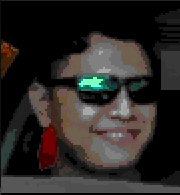
\includegraphics[width=8cm]{face.png}
    \caption{Boot image, a picture of the project author (Raka Gunarto) with 8 bit colour}
\end{figure}
\begin{listing}[H]
    \begin{minted}{c}
static const unsigned int BOOTIMG_WIDTH = 91;
static const unsigned int BOOTIMG_HEIGHT = 96;
static const char BOOTIMG[] = {
    ...
        17,18,234,161,161,161,162,162,163,24,24,24,25,25,25,25,
	25,25,25,25,25,25,25,24,24,24,24,24,162,162,162,162,
	162,162,162,162,162,161,235,234,233,17,0,0,0,0,17,17,
	17,17,17,17,17,17,18,18,18,18,18,
	185,186,186,186,186,186,209,0,0,0,0,0,0,0,0,0,
	0,0,0,0,0,0,0,0,0,0,0,0,0,0,0,17,
	18,234,234,162,162,162,162,162,24,24,24,24,25,25,25,25,
	25,25,25,25,25,25,24,24,24,24,24,24,162,162,162,162,
	162,162,162,162,162,162,161,235,234,18,0,0,0,0,17,17,
	17,17,17,17,17,17,17,17,17,17,18,
	186,186,186,186,186,186,17,0,0,0,0,0,0,0,0,0,
	0,0,0,0,0,0,0,0,0,0,0,0,17,17,18,18,
	18,233,161,162,162,162,162,162,24,24,24,25,25,25,25,25,
	25,25,25,25,25,25,24,24,24,24,24,24,162,162,162,162,
	162,162,163,162,162,162,161,235,235,233,17,0,0,0,0,0,
    ...
}
    \end{minted}
    \caption{kernel/bootimg.h, code snippet of how the boot image is stored}
\end{listing}
\begin{listing}[H]
    \begin{minted}{c}
  //-- load the bootimage on screen, offset by CPU
  // find how many images fit in a line on the screen
  static const int xfit = 320 / BOOTIMG_WIDTH;

  // figure out the offset for the image based on the CPU id
  const int xoffset = cpu % xfit;
  const int yoffset = cpu / xfit;

  // copy image to screen framebuffer, taking offset into account
  for (int y = 0; y < BOOTIMG_HEIGHT; y++)
    for (int x = 0; x < BOOTIMG_WIDTH; x++)
      vga_framebuffer[(y * 320) + x + (xoffset * BOOTIMG_WIDTH) + (yoffset * 320 * BOOTIMG_HEIGHT)] = BOOTIMG[y * BOOTIMG_WIDTH + x];
  //--
    \end{minted}
    \caption{kernel/vga.c, displaying the bootimage per CPU}
\end{listing}

\section{Window switching code snippet}
\label{appendix:c:6}
\begin{listing}[H]
  \begin{minted}{c}
// uart input interrupts go here
int windowmanintr(int c)
{
    switch (c)
    {
    case C('T'): // control-t switches windows
        if (active_window == ROWS * COLUMNS)
            active_window = 0;
        else
            active_window++;
        drawborders();
        return 0;
        ...
  \end{minted}
  \caption{kernel/windowman.c, handle control character from UART to cycle windows}
\end{listing}

\begin{listing}[H]
  \begin{minted}{c}
static void
drawborders()
{
    const int width = vga_getwidth();
    const int height = vga_getheight();

    const int activewin_row = active_window / COLUMNS;
    const int activewin_col = active_window % COLUMNS;

    // draw vertical lines
    const int xinterval = width / COLUMNS;
    for (int col = 1; col < COLUMNS; ++col)
        for (int y = 0; y < height; ++y)
            if ((col == activewin_col || col - 1 == activewin_col) && (y / (height / ROWS)) == activewin_row)
                vga_putpixel(xinterval * col, y, 0x28);
            else
                vga_putpixel(xinterval * col, y, 0x0F);

    // draw horizontal lines
    const int yinterval = height / ROWS;
    for (int row = 1; row < ROWS; ++row)
        for (int x = 0; x < width; ++x)
            if ((row == activewin_row || row - 1 == activewin_row) && (x / (width / COLUMNS)) == activewin_col)
                vga_putpixel(x, yinterval * row, 0x28);
            else
                vga_putpixel(x, yinterval * row, 0x0F);
}
  \end{minted}
  \caption{kernel/windowman.c, draw window borders, highlight active window in red}
\end{listing}

\section{Window device file functions}
\label{appendix:c:7}
\begin{minted}[breaklines]{c}
// reads max n events from winow event queue, with window specified by the minor
// number in the device file.
// copies a windowevent struct or array into addr,
int windowmanread(int user_dst, uint64 addr, int n, struct file *f)
{
    if (!f)
        return -1;

    if (f->ip->minor >= (ROWS * COLUMNS)) // invalid window
        return -1;

    // find head of event queue
    for (int headidx = 0; headidx < NEVTS; ++headidx)
    {
        // skip if not head
        if (evt_queue[f->ip->minor][headidx].type != HEAD)
            continue;
        
        // return if queue empty
        if (evt_queue[f->ip->minor][(headidx + 1) % NEVTS].type == TAIL)
            return 0;

        // return all events up to n
        evt_queue[f->ip->minor][headidx].type = EVT_KEY; // set to something else, just not HEAD or TAIL
        int evt_count = 0;
        int current_evtidx = (headidx + 1) % NEVTS;
        uint64 caddr = addr;
        for (;
             evt_count < n && evt_queue[f->ip->minor][current_evtidx].type != TAIL;
             current_evtidx = (current_evtidx + 1) % NEVTS,
             ++evt_count,
             caddr += sizeof(struct windowevent))
        {
            either_copyout(user_dst, caddr, &evt_queue[f->ip->minor][current_evtidx], sizeof(struct windowevent));
            evt_queue[f->ip->minor][current_evtidx].type = HEAD;
        }

        return evt_count;
    }

    return 0;
}
\end{minted}
\captionof{listing}{kernel/windowman.c, window device file read function}
\pagebreak
\begin{minted}[breaklines]{c}
// write to window specified by the minor number in the device file.
// bytes are taken from memory specified at addr, length n,
// written to the window starting from the offset in the file struct.
// TODO: some point in the future maybe support bit blitting?
int windowmanwrite(int user_src, uint64 addr, int n, struct file *f)
{
    if (!f)
        return -1;

    if (f->ip->minor >= (ROWS * COLUMNS)) // invalid window
        return -1;

    // check out of bounds
    const int width = vga_getwidth();
    const int height = vga_getheight();
    if (f->off + n > (width / COLUMNS) * (height / ROWS))
        return -1;

    // get framebuffer for direct access
    volatile uint8 *framebuffer = vga_getframebuffer();

    // calculate starting offsets for window
    const int xoffset = (width / COLUMNS) * (f->ip->minor % COLUMNS);
    const int yoffset = (height / ROWS) * (f->ip->minor / COLUMNS);

    // calculate initial offset in window if f->off isn't 0
    int bytes_left = n;
    int current_x = f->off % (width / COLUMNS);
    int current_y = f->off / (width / COLUMNS);

    while (bytes_left > 0)
    {
        // check bytes left will overflow this row
        if (bytes_left + current_x >= (width / COLUMNS))
        {
            either_copyin(
                framebuffer + (xoffset + current_x) + (yoffset + current_y) * width,
                user_src,
                addr,
                (width / COLUMNS) - current_x);
            bytes_left -= (width / COLUMNS) - current_x;
            current_x = 0;
            current_y++;
            continue;
        }

        // fits in this row
        either_copyin(
            framebuffer + (xoffset + current_x) + (yoffset + current_y) * width,
            user_src,
            addr,
            bytes_left);
        bytes_left = 0;
    }

    drawborders();
    return 0;
}
\end{minted}
\captionof{listing}{kernel/windowman.c, window device file write function}

\section{Process priority system call}
\label{appendix:c:8}
\begin{minted}[breaklines]{diff}
--- a/kernel/syscall.c
+++ b/kernel/syscall.c
@@ -105,6 +105,7 @@ extern uint64 sys_unlink(void);
 extern uint64 sys_wait(void);
 extern uint64 sys_write(void);
 extern uint64 sys_uptime(void);
+extern uint64 sys_setpriority(void);
 
 static uint64 (*syscalls[])(void) = {
 [SYS_fork]    sys_fork,
@@ -128,6 +129,7 @@ static uint64 (*syscalls[])(void) = {
 [SYS_link]    sys_link,
 [SYS_mkdir]   sys_mkdir,
 [SYS_seek]    sys_seek,
+[SYS_setpriority]    sys_setpriority,
 [SYS_close]   sys_close,
 };
 
--- a/kernel/syscall.h
+++ b/kernel/syscall.h
@@ -20,4 +20,5 @@
 #define SYS_link   19
 #define SYS_mkdir  20
 #define SYS_seek  20
-#define SYS_close  21
+#define SYS_setpriority  21
+#define SYS_close  22
--- a/kernel/sysproc.c
+++ b/kernel/sysproc.c
@@ -17,6 +17,18 @@ sys_exit(void)
   return 0;  // not reached
 }
 
+uint64
+sys_setpriority(void)
+{
+  int prio;
+  if (argint(0, &prio) < 0)
+    return -1;
+  if (prio != 0 || prio != 1)
+    return -1;
+  myproc()->priority = prio;
+  return 0;
+}
+
 uint64
 sys_getpid(void)
 {
--- a/user/user.h
+++ b/user/user.h
@@ -24,6 +24,7 @@ int getpid(void);
 char* sbrk(int);
 int sleep(int);
 int uptime(void);
+int setpriority(int);
 
 // ulib.c
 int stat(const char*, struct stat*);
diff --git a/user/usys.pl b/user/usys.pl
index 5c787e34826f633b249b63ab338043ea69d64269..2813e432c4dff7703ad5c7203f4cbebb7bbce0e7 100755
--- a/user/usys.pl
+++ b/user/usys.pl
@@ -37,3 +37,4 @@ entry("getpid");
 entry("sbrk");
\end{minted}
\captionof{listing}{Diff at commit da05fd8d to add the setpriority() system call}

\section{High framerate game program code}
\label{appendix:c:9}
\begin{minted}{c}
const int gunsprite_width = 6;
const int gunsprite_height = 8;
const uint8 gunsprite[] =
{
    0x00, 0x00, 0x0B, 0x0B, 0x00, 0x00,
    0x00, 0x00, 0x0C, 0x0C, 0x00, 0x00,
    0x00, 0x0C, 0x0C, 0x0C, 0x0C, 0x00,
    0x00, 0x0C, 0x0C, 0x0C, 0x0C, 0x00,
    0x00, 0x0C, 0x0C, 0x0C, 0x0C, 0x00,
    0x00, 0x0C, 0x0C, 0x0C, 0x0C, 0x00,
    0x0C, 0x0C, 0x0C, 0x0C, 0x0C, 0x0C,
    0x0C, 0x0C, 0x0C, 0x0C, 0x0C, 0x0C,
};

struct coords {
    uint x;
    uint y;
};

static void fire(int bulletx, int bullety, struct coords *bullets)
{
    for (int i = 0; i < 10; ++i)
        if (bullets[i].x == -1 && bullets[i].y == -1)
        {
            bullets[i].x = bulletx, bullets[i].y = bullety;
            break;
        }
}

static int colliding(struct coords c1, struct coords c2, int combinedrad)
{
    uint rsquared = combinedrad * combinedrad;
    uint dx = c1.x - c2.x;
    uint dy = c1.y - c2.y;
    uint distsquared = dx * dx + dy * dy;
    if (distsquared <= rsquared)
        return 1;
    return 0;
}

int main(int argc, char *argv[])
{
    setpriority(1);

    // open the first available window
    window_handle win = window_create();

    struct windowevent evt;
    struct window_dim dim = window_getdimensions(win);

    int gunx = dim.width / 2;
    int guny = (dim.height / 4) * 3;

    const uint bulletrad = 3;
    struct coords bullets[10];

    const uint enemywh = 5;
    struct coords enemies[10];

    for(int i = 0; i < 10; ++i)
    {
        bullets[i].x = -1;
        bullets[i].y = -1;

        int row = i / 5 + 1;
        enemies[i].x = ((i % 5) + row) * (dim.width / 6);
        enemies[i].y = row * (dim.height / 4);
    }
    
    uint score = 0;
    while (score < 10)
    {
        // clear screen
        window_clearscreen(win);

        // handle inputs
        if (window_pollevent(win, &evt, 1) == 1)
        {
            switch (evt.payload)
            {
            case 'a':
                gunx = gunx > 0 ? gunx - 1 : gunx;
                break;
            case 'd':
                gunx = gunx < dim.width ? gunx + 1 : gunx;
                break;
            case ' ':
                fire(gunx + gunsprite_width, guny - 2, bullets);
                break;
            default:
                break;
            }
        }

        // movement
        for(int i = 0; i < 10; ++i)
        {
            // bullets, delete when top of screen reached
            if (bullets[i].x != -1 && bullets[i].y != -1)
                if (--bullets[i].y <= 0)
                    bullets[i].x = -1, bullets[i].y = -1;


        }

        // collisions
        for(int bullet = 0; bullet < 10; ++bullet)
            if (bullets[bullet].x != -1 && bullets[bullet].y != -1)
                for (int enemy = 0; enemy < 10; ++enemy)
                    if (enemies[enemy].x != -1 && enemies[enemy].y != -1 && colliding(bullets[bullet], enemies[enemy], bulletrad + enemywh / 2))
                    {
                        score++;
                        bullets[bullet].x = -1, bullets[bullet].y = -1;
                        enemies[enemy].x = -1, enemies[enemy].y = -1;
                        break;
                    }

        // draw
        window_drawsprite(win, gunx, guny, gunsprite_width, gunsprite_height, gunsprite);
        for(int i = 0; i < 10; ++i)
        {
            if (bullets[i].x != -1 && bullets[i].y != -1)
                window_drawcircle(win, bullets[i].x - bulletrad, bullets[i].y - bulletrad, bulletrad, 0x0C);
            
            if (enemies[i].x != -1 && enemies[i].y != -1)
                window_drawrect(win, enemies[i].x - enemywh, enemies[i].y - enemywh, enemywh, enemywh, 0x0E);
        }

        window_drawchar(win, 8*0, 0, 'S', 0x09);
        window_drawchar(win, 8*1, 0, 'C', 0x09);
        window_drawchar(win, 8*2, 0, 'O', 0x09);
        window_drawchar(win, 8*3, 0, 'R', 0x09);
        window_drawchar(win, 8*4, 0, 'E', 0x09);
        window_drawchar(win, 8*5, 0, ':', 0x09);
        window_drawchar(win, 8*6, 0, ' ', 0x09);
        window_drawchar(win, 8*7, 0, (char)score + 48, 0x09);
    }
    window_destroy(win);
    exit(0);
}
\end{minted}
\captionof{listing}{user/game.c source code}

\end{appendices}
